\documentclass[11pt]{article}
\usepackage{lamba_tr}
\usepackage{amsmath,amssymb}
\usepackage{booktabs}
\usepackage{multirow}
\usepackage{array}
\usepackage{enumitem}
\usepackage{caption}
\usepackage{subcaption}
\usepackage[numbers,sort&compress]{natbib}
\usepackage{algorithm}
\usepackage{algpseudocode}
\usepackage{bm}
\setlist{itemsep=0.15em,topsep=0.3em}
\captionsetup{font=small,labelfont=bf}
\setlength{\emergencystretch}{3em}
\hypersetup{pdftitle={Lamba: Reducing Doom Loops and Answer-Letter Bias Without Losing Capability},
  pdfauthor={Vixero Labs}, pdfsubject={Technical Report of Lamba 0.1 and 0.2}}

\newcommand{\Rany}{R_{\text{any}}}
\newcommand{\Rheavy}{R_{\text{heavy}}}
\newcommand{\todo}[1]{\textcolor{red}{[TODO: #1]}}

\title{Lamba: Reducing Doom Loops and Answer-Letter Bias Without Losing Capability}
\subtitle{Technical Report of Lamba 0.1 and 0.2}
\shorttitle{Lamba: Reducing Doom Loops and Answer-Letter Bias}
\author{Vixero Labs}
\date{Snapshot of 2 October 2026}

\begin{document}
\maketitle

\begin{abstract}
We describe Lamba 0.1 and Lamba 0.2, two LoRA adapters on a 28.8B-parameter hybrid model from the Qwen3.5 family (48 Gated DeltaNet and 16 full-attention layers), built by one researcher on a single GPU. The base model had two defects: it falls into runaway repetition (``doom loops'') on long reasoning, and on the Malay benchmark MalayMMLU it is 11.2 points less accurate when the answer is A than when it is B. Lamba 0.1 adapts Liquid AI's AntiDoom recipe to this architecture, mines loops from its own outputs and per language, and adds a separate letter-bias stage. On our 150-prompt loop test, runaway loops at the end of answers fall from 18.0\% to 0\%, and any repetition in the final 2,500 characters from 37.3\% to 2.7\%. A factorial comparison shows that training alone and a repetition penalty of 1.1 alone each remove most loops, by similar amounts; combined they leave the fewest loops, but on our pre-registered primary endpoint (exact repetition or token-budget exhaustion) all three give a similar improvement of about 25\% relative on 700 prompts, short of the 30\% we targeted. The A--B gap shrinks from $-11.2$ to $-1.9$ points on the full 23,903-item benchmark, although the checkpoint was chosen on that benchmark. GPQA-Diamond and MalayMMLU accuracy show no significant change. Lamba 0.2 adds a DPO stage on tool-use transcripts and shows no significant difference from Lamba 0.1 on the metrics we tested. We compare against eight other models on the same test sets and report the full lineage, the negative results, and the corrections we made to our own measurements.
\end{abstract}

\setcounter{tocdepth}{1}
\tableofcontents
\newpage

%=====================================================================
\section{Introduction}
%=====================================================================

Reasoning models fail in a characteristic way: they start repeating a sentence, a list item or a line of arithmetic and do not stop until the token budget runs out. Liquid AI called these \emph{doom loops} and showed that a preference-optimisation method applied at the token where a repeat begins (AntiDoom, built on final-token preference optimisation, FTPO) removes most of them in small models \citep{liquid2025antidoom}. Our base model, a further-trained checkpoint of the Qwen3.5 architecture, loops often: on our held-out loop test, 39.3\% of greedy answers contain a block of at least 60 characters repeated four or more times, and 18.0\% end in a runaway loop.

The same model carries a positional prior on MalayMMLU \citep{malaymmlu}: when the correct answer is A it is right 71.6\% of the time, when it is B, 82.9\%. Moving the gold answer between positions shows this is a preference for answer positions, not a content effect.

Lamba is the work of one researcher at Vixero Labs, on one NVIDIA L40S. The first training run was on 19 September 2026; Lamba 0.1 shipped on 23 September and Lamba 0.2 on 2 October. Figure~\ref{fig:method} shows how a training pair is built from a looping output, and Figure~\ref{fig:lineage} how each training stage changed loop behaviour.

\begin{figure}[t]
  \centering
  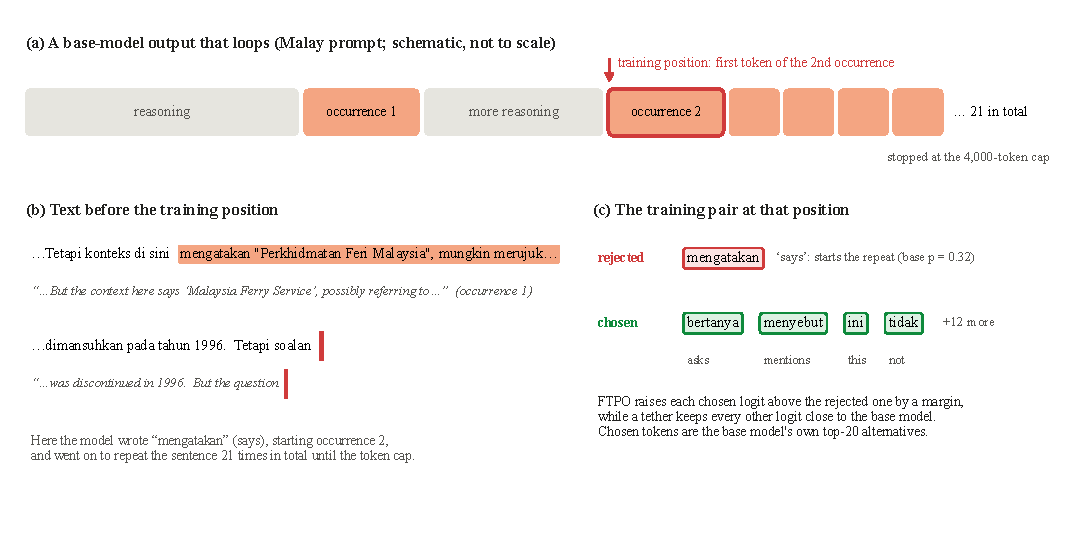
\includegraphics[width=\linewidth]{figures/method.pdf}
  \caption{How an AntiDoom training pair is built, shown on a real pair from our training data. (a) The base model repeats a sentence 21 times and runs out of tokens. (b) The context is cut at the first token of the second occurrence. (c) The token the model actually produced there is rejected; the base model's own top alternatives are chosen. Glosses are English translations of the Malay.}
  \label{fig:method}
\end{figure}

\begin{figure}[t]
  \centering
  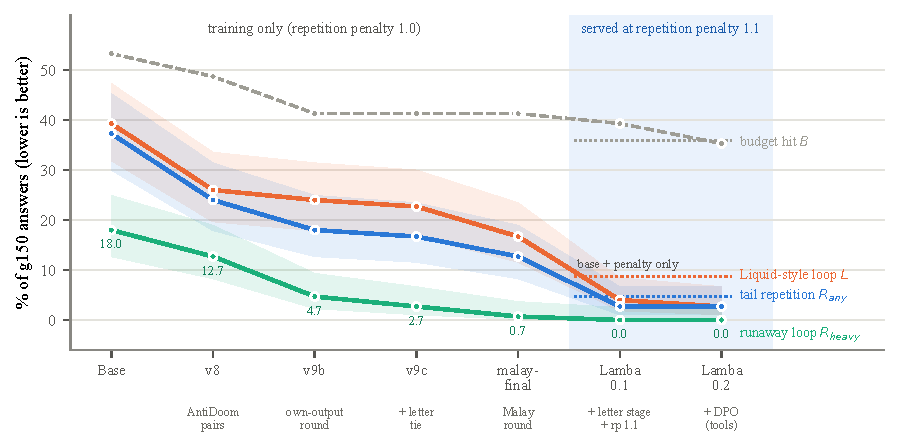
\includegraphics[width=\linewidth]{figures/lineage.pdf}
  \caption{Loop rates on the 150-prompt loop test (g150) across the Lamba lineage, recomputed from raw outputs; shaded bands are 95\% Wilson intervals. The first five points are evaluated without a repetition penalty, so they isolate the effect of training: runaway loops ($\Rheavy$) fall from 18.0\% to 0.7\%. The shaded points are the shipped versions, served at repetition penalty 1.1; dotted lines mark the untouched base model with the same penalty, which achieves most of the same reduction on its own (\S\ref{sec:decoding}). Budget hits (dashed) fall less because many \texttt{mcp} prompts need long but legitimate solutions (Table~\ref{tab:domain}).}
  \label{fig:lineage}
\end{figure}

\paragraph{Contributions.}
\begin{itemize}
  \item \textbf{AntiDoom on a hybrid model.} We port AntiDoom to a 28.8B Gated DeltaNet hybrid, with an architecture-aware LoRA layout, mining on the adapter's own outputs, and a per-language round built from model-written prompts for a domain where natural loops are too rare to mine (\S\ref{sec:loops}).
  \item \textbf{Training versus decoding.} A $2\times2$ comparison (base or adapter, with or without a repetition penalty) on 700 prompts shows that training alone and the penalty alone are about equally effective, and that combining them removes the most loops ($\Rany$: 225 base, 47 training only, 37 penalty only, 14 both). A penalty of 1.2 makes loops worse than the base model (\S\ref{sec:decoding}).
  \item \textbf{Letter bias and checkpoint instability.} A group objective over cyclic option rotations reduces the A--B gap from $-11.2$ to $-1.9$ points, and we document that letter-bias checkpoints of a single run range from $-13.7$ to $+11.7$ points on the full benchmark (\S\ref{sec:letters}).
  \item \textbf{Measurement.} A frozen metric for redundant tool calls after a verified answer; the finding that most of Lamba 0.1's tool failures came from the evaluation sandbox, not the model; and a pre-registered loop endpoint reported under both the planned and a substituted detector (\S\ref{sec:eval}, \S\ref{sec:tools}).
  \item \textbf{An open record.} Results for eight other models on the same harness (\S\ref{sec:compare}), every negative result (\S\ref{sec:negative}), the corrections we made along the way (Appendix~\ref{app:retractions}), and the code for the trainer, the loop and tool evaluations and the scorers.
\end{itemize}

\paragraph{Key findings.}
\begin{enumerate}
  \item \emph{Training and the penalty are interchangeable, and complementary.} On 700 prompts, training alone cuts runaway loops from 16.6\% to 1.0\% and the penalty alone to 0.3\%; together they leave 2.0\% tail repetition against 6.7\% and 5.3\% for each alone. On budget hits and the primary endpoint the three configurations are indistinguishable (\S\ref{sec:decoding}).
  \item \emph{Learning from re-quoting loops generalises.} 80\% of the first-round training pairs come from loops in which the model re-quotes the question, yet our evaluation, which ignores text copied from the prompt, shows loops in the model's own words falling sharply, including on science and Malay prompts with little overlap with training data (\S\ref{sec:analysis}).
  \item \emph{The training position is everything.} One position earlier than the start of the repeat, the same pipeline taught the model to stop writing newlines and made loops worse (\S\ref{sec:analysis}).
  \item \emph{The useful penalty window is narrow.} At 1.2 the penalty pushes 87\% of answers into the token cap, against 41\% without it (\S\ref{sec:analysis}).
  \item \emph{Results replicate across seeds.} Retraining the last loop stage with a new seed changes no loop or capability metric significantly (\S\ref{sec:analysis}).
  \item \emph{Bias checkpoints are unstable.} Seven checkpoints of one letter-bias run range from $-13.7$ to $+11.7$ points (\S\ref{sec:letters}).
\end{enumerate}

When given its system prompt, Lamba introduces itself as ``Lamba, built by Vixero Labs''. It is built on a Qwen-family base, and its model card says so.

%=====================================================================
\section{Related work}
%=====================================================================

\paragraph{Repetition in neural text generation.} Greedy and beam decoding produce repetitive text even from strong language models \citep{holtzman2020degeneration}. Training-time remedies penalise repeated tokens directly, as in unlikelihood training \citep{welleck2020unlikelihood}, or teach the model to escape sentence-level loops using synthetic repetitive data, as in DITTO \citep{xu2022ditto}, which also showed that repetitions reinforce themselves. Decode-time remedies include the repetition penalty introduced with CTRL \citep{keskar2019ctrl}, which we use, and nucleus sampling. AntiDoom \citep{liquid2025antidoom} targets the long loops of reasoning models with a single-token preference objective at the start of the first repeat. We follow it closely, scale it to a 28.8B hybrid model, and measure how much of the gain comes from training and how much from the penalty.

\paragraph{Answer-position bias.} Multiple-choice accuracy of language models changes when options are reordered \citep{pezeshkpour2024order}, largely because of a prior over option identifiers \citep{zheng2024pride}. Proposed fixes include inference-time debiasing \citep{zheng2024pride}, fine-tuning on permutation-consistency objectives with LoRA \citep{lora1_pbm} and reinforcement learning that rewards consistent answers across permutations \citep{pagrpo}. Our letter stage is a supervised group objective in the same family, applied to a Malay benchmark.

\paragraph{Efficient reasoning.} Reasoning models often spend many tokens on problems that need few \citep{chen2024overthinking}. ThinkingCap \citep{thinkingcap} fine-tunes the same base architecture as Lamba for shorter reasoning, and we compare against it directly. Our own efficiency experiments were negative or inconclusive (\S\ref{sec:negative}), and we leave verbosity to future work.

%=====================================================================
\section{Setup}
%=====================================================================

\paragraph{Base model.} The base (\texttt{soup-linear-l1.0}) is a 28.8B-parameter model with the architecture of Qwen3.8-27B \citep{qwen38}: 64 layers, hidden size 5120, 48 Gated DeltaNet layers \citep{yang2025gdn} interleaved with 16 full-attention layers. We continued training it before this work and treat it as fixed here.

\paragraph{Hardware.} All training and evaluation ran on a single NVIDIA L40S (48\,GB, about 46\,GB usable) with 30\,GB of host RAM; a second identical machine was used on a few days for evaluation. The base cannot be held in bf16 on the card, so training uses 4-bit (NF4) QLoRA \citep{dettmers2023qlora} and serving uses online fp8 quantisation. Appendix~\ref{app:compute} gives run times.

\paragraph{Software.} vLLM 0.28 \citep{kwon2023vllm} for generation, with multi-token-prediction speculative decoding (3 tokens) and the Qwen3 reasoning and XML tool-call parsers; PyTorch 2.11 with CUDA 13.4; fused Gated DeltaNet kernels (\texttt{fla-core} 0.5.2, \texttt{causal-conv1d} 1.7.0), which cut training step time from 405\,s to 131\,s; and a trainer derived from Liquid AI's AntiDoom code with our own losses.

\paragraph{Adapter scheme.} LoRA \citep{hu2022lora} with per-module ranks: 128 on attention $q,k,v,o$; 64 on MLP projections; 64 on the Gated DeltaNet input projection for $q,k,v$, 32 on its gate projection, 64 on its output projection; 16 on the LM head. Adapters cover all 16 full-attention layers and the last 24 Gated DeltaNet layers. vLLM cannot apply LoRA to the LM head, so we merge only the LM-head delta, with stochastic rounding, into a copy of that weight. Per-stage hyperparameters are in Appendix~\ref{app:hparams}.

\paragraph{Why the adapter is not merged.} For our adapters the fp8 quantisation noise is three to eight times the size of the LoRA delta under every rounding scheme we tried, so merging would erase it. vLLM computes the base output and the LoRA correction separately, so serving the unmerged adapter on the fp8 base preserves the delta. Every evaluation in this report uses that path.

\paragraph{Decoding.} Loop and capability evaluations are greedy. Lamba and its base run at reasoning effort ``medium'' in every evaluation; the GPQA prompts additionally carry the harness's ``xhigh'' instruction text, identically for the base and all adapters. Lamba is served with repetition penalty 1.1 unless stated otherwise. Single-stream serving runs at 14.8 tokens/s without speculative decoding and 41.6 tokens/s with three draft tokens.

%=====================================================================
\section{Method}
\label{sec:method}
%=====================================================================

All training objectives act on the next-token logits at a single position. We write $\bm{z}\in\mathbb{R}^{V}$ for the adapter's logits, $\bm{z}^{0}$ for the logits of the frozen base model (the same network with the adapter disabled), and $p_\theta = \mathrm{softmax}(\bm{z})$, $p_0 = \mathrm{softmax}(\bm{z}^{0})$.

\paragraph{Mining loop pairs.} Algorithm~\ref{alg:mining} turns a looping output into a preference pair (Figure~\ref{fig:method}). The position is the first token of the second occurrence of the repeated unit; the rejected token $r$ is what the model produced there, and the chosen set $C$ is the base model's top-20 alternatives at the same context.

\begin{algorithm}[t]
\caption{Mining AntiDoom pairs from model outputs}
\label{alg:mining}
\small
\begin{algorithmic}[1]
\Require outputs $\mathcal{Y}$ with prompts; base model $f_0$; window $w{=}60$ characters; minimum count $k{=}4$
\For{each output $y$ with prompt $x$}
  \State $\mathcal{W} \gets$ windows of $w$ characters, anchored every $w/2$, with $\geq$25 alphanumeric characters, occurring $\geq k$ times in $y$ without overlap
  \For{each repeated window in $\mathcal{W}$}
    \State $p_1 \gets$ start of its second occurrence; $p_0 \gets$ start of its first
    \State extend $p_0, p_1$ leftward while $y[p_0{-}1] = y[p_1{-}1]$, then snap $p_1$ to the next word start
    \State $c \gets x \oplus y[{:}p_1]$ \Comment{context ends just before the repeat}
    \State $r \gets$ first token of $y[p_1{:}]$ \Comment{rejected: starts the repeat}
    \State $C \gets$ top-20 tokens of $f_0(c)$ other than $r$, excluding non-alphanumeric tokens
    \If{$\log p_0(r) < -0.5$ \textbf{and} $\max_{t\in C}\log p_0(t) - \log p_0(r) > -5$}
      \State keep $(c, r, C)$ \Comment{skip near-certain repeats; require a plausible alternative}
    \EndIf
  \EndFor
\EndFor
\State keep at most two pairs per output; cap pairs per rejected token; remove duplicates
\end{algorithmic}
\end{algorithm}

\paragraph{FTPO objective.} For a pair $(c, r, C)$ let $\Delta_t = z_t - z_r$ for each chosen token $t \in C$, and $w_t = \mathrm{clip}\big((\varepsilon - \Delta_t)/\varepsilon,\,0,\,1\big)$ with margin $\varepsilon = 1.5$. The preference loss pushes every chosen logit above the rejected one by the margin and stops pushing once it is reached:
\begin{equation}
\mathcal{L}_{\text{pref}} = \frac{1}{|C|}\sum_{t\in C} w_t\,\mathrm{softplus}\big(\varepsilon - \Delta_t\big).
\label{eq:ftpo}
\end{equation}
A tether keeps all other logits close to the base model and limits how far the target logits move:
\begin{equation}
\mathcal{L}_{\text{tether}} = \lambda \operatorname*{mean}_{v\notin C\cup\{r\}} \big(z_v - z^{0}_v\big)^2 \;+\; \lambda_t \operatorname*{mean}_{v\in C\cup\{r\}} \max\!\big(|z_v - z^{0}_v| - \tau_t,\,0\big)^2,
\label{eq:tether}
\end{equation}
with $\lambda = 2.0$ for v8 and $0.1$ afterwards, $\lambda_t = 0.1$ and $\tau_t = 0.1$. The loss for a hard pair is $\mathcal{L}_{\text{pref}} + \mathcal{L}_{\text{tether}}$.

\paragraph{Soft rows.} Later occurrences of a repeat, and contexts where the base model is nearly certain of the repeated token, use a soft target instead of a hard pair:
\begin{equation}
q = \tfrac12\,p_0 + \tfrac12\,\mathrm{softmax}\!\Big(\frac{\log p_0 - \gamma\,\bm{e}_r}{\tau}\Big), \qquad \mathcal{L}_{\text{soft}} = \omega\;\mathrm{KL}\big(q \,\|\, p_\theta\big),
\label{eq:soft}
\end{equation}
where $\bm{e}_r$ is the indicator of the rejected token, $\gamma=4$, $\tau=0.7$, and $\omega \leq 1$ is a per-row weight. With $\gamma=0$ and $\tau=1$ the target is $q = p_0$; we use such rows to tie the adapter to the base model on non-looping text and on answer letters.

\paragraph{Letter-group objective.} A training example is a group of $K$ renderings of one question, each a cyclic rotation $\pi_k$ of the options. In rendering $k$ the chosen token is the gold letter $g_k$ and the rejected token $\bar{g}_k$ is the base model's highest-scoring wrong letter. With $\bm{a}_k$ the probabilities over the option letters and $\tilde a_{k,j}$ the probability given to original option $j$ (undoing $\pi_k$),
\begin{equation}
\mathcal{L}_{\text{letter}} = \alpha\,\frac1K\sum_k w_k\,\mathrm{softplus}\big(\varepsilon - (z_{k,g_k} - z_{k,\bar g_k})\big)
+ \lambda_{\text{pv}}\,\frac1n\sum_{j}\operatorname*{var}_k\big(\log \tilde a_{k,j}\big)
+ \lambda_H\,\frac1K\sum_k H(\bm{a}_k)
+ \lambda\,\mathcal{L}_{\text{tether}}^{\neg\text{letters}},
\label{eq:letter}
\end{equation}
where the second term penalises the same option receiving different probability under different rotations, the entropy term discourages flat letter distributions, and the tether excludes all option letters. Lamba 0.1 uses $\alpha = 0.4$, $\lambda_{\text{pv}} = 0.2$, $\lambda_H = 0.05$.

\paragraph{DPO stage.} Lamba 0.2 adds the standard DPO loss \citep{rafailov2023dpo} on full responses, combined with the terms listed in \S\ref{sec:tools}.

%=====================================================================
\section{Evaluation protocol}
\label{sec:eval}
%=====================================================================

\subsection{Loop test}

The main loop test (g150) is 150 loop-prone prompts that were never used to build training pairs: 65 from the \texttt{mcp} domain, 65 science and 20 Malay\footnote{\texttt{mcp}: competition mathematics and competitive programming problems from our internal corpus.}. Many \texttt{mcp} prompts share templated wording with training prompts (60 of 65 have at least 50\% 8-gram overlap with some training prompt); science and Malay prompts have little overlap, and the loop reduction holds on them separately (Table~\ref{tab:domain}). Generation is greedy with a 4,000-token cap that includes the reasoning. For each output we compute:

\begin{itemize}
  \item $L$ (Liquid-style loop): some window of $\geq$60 characters (with $\geq$25 alphanumeric) occurs $\geq$4 times anywhere in the output.
  \item $\Rany$: any such repeated text inside the last 2,500 characters.
  \item $\Rheavy$: more than 1,500 repeated characters inside the last 2,500 characters, i.e.\ a runaway loop at the end.
  \item $B$ (budget hit): generation stopped at the 4,000-token cap.
\end{itemize}

Windows that also occur in the prompt are excluded, so quoting the question is not counted. Comparisons are paired by prompt and tested with an exact McNemar test; confidence intervals on relative reductions use 2,000 bootstrap resamples over prompts. These detectors are from the same family as the one used to mine training pairs, so we also ran two independent checks on earlier adapters in the lineage: a zlib compression-ratio test with no repetition detector (on v8) and blind adjudication of 40 output pairs by a separate model (on v9c: 10 base outputs and 1 adapter output judged to end in a runaway loop, $p=0.004$). Both agreed in direction.

\paragraph{Pre-registered endpoint.} Before any training we fixed the success rule: on held-out loop-prone prompts, the rate of \emph{exact repetition or budget hit} must fall with one-sided McNemar $p<0.025$, by at least 30\% relative and at least 10 points absolute. ``Exact repetition'' is defined by the inner-repetition detector shipped with the AntiDoom code. The original rule also counted a semantic near-duplicate detector; after seeing base-model data, and before seeing any adapter data, we removed it because it fired on 69 of 70 base outputs. Later in the project, internal analyses computed the same endpoint with the Liquid-style detector $L$ in place of the inner-repetition detector. That substitution was not a planned change, and we report both versions (Table~\ref{tab:primary}).

\subsection{Other evaluations}

\begin{itemize}
  \item \textbf{GPQA-Diamond} \citep{rein2023gpqa}: 198 questions from an ungated mirror containing the same problems, greedy, 4,000-token budget with a forced answer at the cap. Between 51\% and 59\% of answers are cut at the cap depending on the model, so absolute accuracy is a proxy and we only compare at equal budgets.
  \item \textbf{MalayMMLU} \citep{malaymmlu}: all 23,903 items whose gold answer is A--D, scored by the log-probability of the answer-letter token. We report accuracy, position-balanced accuracy (mean of per-gold-letter accuracy), the A--B accuracy gap, the standard deviation of per-position recall (RStd) and a calibration divergence (CKLD) following \citet{zheng2024pride}.
  \item \textbf{Shift test}: 5,000 MalayMMLU items under every cyclic rotation of the options; consistency is the share of questions answered with the same content under all rotations, and shift-RStd is the spread of accuracy across positions.
  \item \textbf{eval30}: 30 maths tasks with sympy-verified answers (12 definite integrals and 18 across ODEs, series, linear systems, limits, combinatorics and matrices), 8 runs each at temperature 0.8, with a Python tool in a sandbox and at most 8 tool rounds, scored with a frozen metric (\S\ref{sec:tools}).
\end{itemize}

We report many paired tests without correction for multiple comparisons; isolated results with $0.01<p<0.05$ should be read as weak evidence.

%=====================================================================
\section{Loop reduction}
\label{sec:loops}
%=====================================================================

\subsection{What did not work first}

Our first attempt mined preference pairs from existing base-model rollouts and trained FTPO on them. It had no effect, and later versions made loops worse. Two bugs explain this. The miner used the first occurrence of a repeated span as the training position rather than the start of the second occurrence, so the ``rejected'' tokens were ordinary text: 15\% were the paragraph break \verb|\n\n| and many others were sentence openers such as ``Then'' and ``The''. Training suppressed newlines (from 7.11 to 0.03 per 1,000 characters) and produced run-on text that looped more. In addition, 89\% of the pairs came from a semantic-similarity detector that fired on 76\% of all rollouts, so most of them were not loops.

\subsection{AntiDoom, as specified}

The version that worked follows Liquid AI's recipe \citep{liquid2025antidoom}. A loop is a 60-character window repeated at least four times. The training position is the first token of the \emph{second} occurrence of the repeated unit (the first repeat), after extending the match leftward to its true start and snapping to a word boundary. The rejected token is the one the model produced there; chosen tokens are the base model's top-20 alternatives, excluding non-alphanumeric tokens.

From 81,661 existing rollouts this gave 22,023 loop events. We kept pairs where the base model was not already near-certain of the rejected token (log-probability below $-0.5$) and the best alternative was within 5 nats, leaving 1,298 pairs. This adapter (v8) was the first with a clear effect: on 586 prompts not used for training, the Liquid-style loop rate fell from 52\% to 32\% ($p=7\times10^{-16}$), while the worst runaway loops at the end of outputs changed little (Figure~\ref{fig:lineage}).

\subsection{Rounds on the adapter's own outputs}

Round 2 mined new loops from v8's outputs on prompts disjoint from all evaluation sets. The second occurrence of each loop became a hard FTPO pair (Eqs.~\ref{eq:ftpo}--\ref{eq:tether}); the third and fourth became soft rows (Eq.~\ref{eq:soft}). 909 mined rows plus 120 rows tying the adapter to the base on non-looping text trained v9b, starting from v8. This is the round that removed most runaway loops ($\Rheavy$ 12.7\% $\rightarrow$ 4.7\%). v9c added 1,080 rows tying answer-letter probabilities to the base on multiple-choice prompts, because v9b had shifted the letter prior (MalayMMLU fell by 1 point). The tie cost nothing on loops and restored MalayMMLU.

\subsection{Malay round}

v9c reduced loops on the domains it was mined from, but on 180 unseen Malay multiple-choice prompts the reduction was small and not significant. Real Malay prompts loop rarely (3.4\%), so mining them gave too few pairs. We had a separate model write Malay prompts likely to elicit loops, ran our own model on them (about 15\% looped) and mined pairs from those outputs. The mix was 273 Malay rows, 600 replay rows from earlier rounds and 200 letter-tie rows, trained for one epoch from v9c. On 400 held-out Malay prompts this adapter (malay-final) reduced $\Rany$ from 7.8\% to 2.5\% and $\Rheavy$ from 5.2\% to 1.5\% ($p<0.001$). On the 180 of those prompts with gradable answers, accuracy rose from 90.6\% to 94.4\%, mostly because fewer answers were cut off.

\subsection{Training versus decoding}
\label{sec:decoding}

To separate what training contributes from what the decoding setting contributes, we ran both the base model and malay-final (the last loop-training stage before the letter stage) with and without repetition penalty 1.1, on g150 and on the 700-prompt set (Table~\ref{tab:decoding}).

\begin{itemize}
  \item \textbf{Each alone removes most loops.} On 700 prompts, training alone takes runaway loops from 116 to 7 and tail repetition from 225 to 47; the penalty alone takes them to 2 and 37. The two are comparable, with the penalty slightly ahead on the loop metrics.
  \item \textbf{Combined is best on loops.} Adding training on top of the penalty roughly halves the loops that remain: Liquid-style loops 52 $\rightarrow$ 21 ($p=9\times10^{-5}$) and tail repetition 37 $\rightarrow$ 14 ($p=4\times10^{-4}$).
  \item \textbf{Budget hits do not care which.} Training only, penalty only and both give 274, 271 and 280 budget hits out of 700 (base: 364). Most remaining budget hits are long but legitimate solutions (Table~\ref{tab:domain}), which neither lever addresses.
\end{itemize}

The practical upshot is that training makes the model loop-resistant without depending on a decoding setting that users may not apply, and the penalty, which costs nothing, adds a further reduction when it is applied. The capability cost of the penalty on the base model is untested; with the adapters, GPQA-D and MalayMMLU are unchanged (Table~\ref{tab:versions}).

\begin{table}[t]
\centering
\small
\caption{Training versus decoding: base model and malay-final, each with and without repetition penalty 1.1 (counts). Paired exact McNemar tests in the text.}
\label{tab:decoding}
\setlength{\tabcolsep}{5pt}
\begin{tabular}{llcccc}
\toprule
Test set & Configuration & $L$ & $\Rany$ & $\Rheavy$ & $B$ \\
\midrule
\multirow{4}{*}{g150 (150)} & Base, no penalty & 59 & 56 & 27 & 80 \\
 & Base + penalty only & 13 & 7 & 0 & 54 \\
 & Training only (malay-final) & 25 & 19 & 1 & 62 \\
 & Training + penalty & 6 & 2 & 0 & 55 \\
\midrule
\multirow{4}{*}{700 prompts} & Base, no penalty & 248 & 225 & 116 & 364 \\
 & Base + penalty only & 52 & 37 & 2 & 271 \\
 & Training only (malay-final) & 69 & 47 & 7 & 274 \\
 & Training + penalty & 21 & 14 & 1 & 280 \\
\bottomrule
\end{tabular}
\end{table}

A sweep of the penalty on top of malay-final (Figure~\ref{fig:rp}) shows a narrow useful window: 1.1 helps, 1.15 helps less than no penalty with the Liquid-style detector and barely at all with the pre-registered one, and 1.2 produces more loops than the base model. Outputs at 1.1 remain coherent and well formatted; newline frequency drops by about 30\%. The penalty was chosen on g150, so g150 results at 1.1 are not an independent test of it.

\subsection{The primary endpoint}

Table~\ref{tab:primary} gives the primary endpoint, against the base model without a penalty, under both detectors. With the pre-registered detector every configuration improves significantly, but on the 700-prompt set (never used for training or for choosing the penalty, although earlier adapters had been evaluated on it) training only, penalty only and both together all land between 22.8\% and 25.3\% relative, below the 30\% target. The point estimates above 30\% occur only on g150, where the penalty was selected. On top of the penalty, the adapters do not change the endpoint at all (relative change $-3.3\%$ on 700 prompts, CI $-11.6$ to $3.9$). The endpoint is dominated by budget hits, many of which are long but legitimate solutions (Table~\ref{tab:domain}), which is why it moves much less than the loop metrics.

\begin{table}[t]
\centering
\small
\caption{Primary endpoint (exact repetition or budget hit), each configuration paired against the base model without a penalty. ``Pre-reg.'' uses the pre-registered inner-repetition detector; ``Liquid'' substitutes the Liquid-style detector $L$. Relative reductions with 95\% bootstrap CIs.}
\label{tab:primary}
\footnotesize
\setlength{\tabcolsep}{3.5pt}
\begin{tabular}{llccc}
\toprule
Configuration & Test set & Pre-reg. rate & Rel., pre-reg. & Rel., Liquid \\
\midrule
Penalty only (base, rp 1.1) & g150 & 53.3 $\rightarrow$ 36.0 & 32.5\% (18.8--45.3) & 34.1\% (22.2--45.8) \\
Training only (malay-final) & g150 & 53.3 $\rightarrow$ 41.3 & 22.5\% (8.7--35.8) & 23.1\% (10.9--35.1) \\
Lamba 0.1 (rp 1.1) & g150 & 53.3 $\rightarrow$ 39.3 & 26.3\% (12.5--38.6) & 33.0\% (19.8--44.9) \\
Lamba 0.2 (rp 1.1) & g150 & 53.3 $\rightarrow$ 35.3 & 33.8\% (18.8--47.6) & 39.6\% (26.0--52.1) \\
\midrule
Penalty only (base, rp 1.1) & 700 prompts & 52.0 $\rightarrow$ 38.9 & 25.3\% (19.5--31.2) & 29.5\% (24.1--35.3) \\
Training only (malay-final) & 700 prompts & 52.0 $\rightarrow$ 39.3 & 24.5\% (18.7--30.1) & 28.5\% (23.5--33.9) \\
Training + penalty (rp 1.1) & 700 prompts & 52.0 $\rightarrow$ 40.1 & 22.8\% (16.6--28.5) & 31.2\% (25.7--37.0) \\
\bottomrule
\end{tabular}
\end{table}

\begin{keybox}
\textbf{Summary of the loop result.} Training alone and a repetition penalty alone each remove most loops, by similar amounts; combined they leave the fewest ($\Rany$ 2.0\% and $\Rheavy$ 0.1\% on 700 prompts, from 32.1\% and 16.6\%). The pre-registered primary endpoint improves by about 25\% relative under any of the three configurations, short of the 30\% target, because it is dominated by long but legitimate answers that hit the token cap.
\end{keybox}

\begin{figure}[t]
  \centering
  \begin{minipage}[t]{0.48\linewidth}
    \centering
    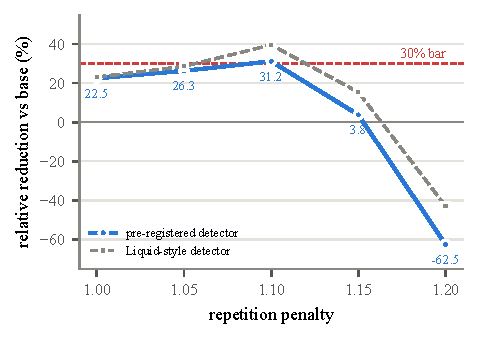
\includegraphics[width=\linewidth]{figures/rp_sweep.pdf}
    \caption{Primary-endpoint reduction versus base for malay-final on g150, by repetition penalty, under both detectors. The penalty was selected from this sweep.}
    \label{fig:rp}
  \end{minipage}\hfill
  \begin{minipage}[t]{0.48\linewidth}
    \centering
    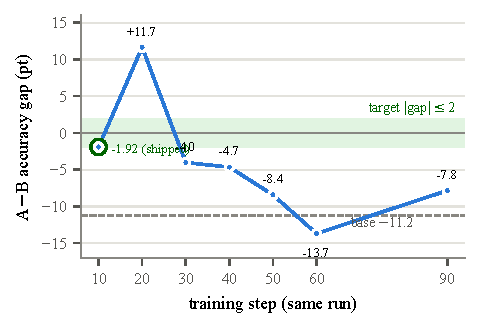
\includegraphics[width=\linewidth]{figures/letter_checkpoints.pdf}
    \caption{A--B gap on the full MalayMMLU for seven checkpoints of one letter-bias run.}
    \label{fig:letters}
  \end{minipage}
\end{figure}

%=====================================================================
\section{Answer-letter bias}
\label{sec:letters}
%=====================================================================

\paragraph{Diagnosis.} On the base model, accuracy by gold letter is 71.6 / 82.9 / 75.5 / 81.3 for A--D. Rotating the options moves the error with the position, and placing options inline instead of on separate lines reverses the pattern, so the bias is a position prior tied to the prompt format, consistent with \citet{zheng2024pride}. Averaging over permutations at inference gives 79.9\%, an upper bound on what removing position effects alone could recover.

\paragraph{Data.} We used multiple-choice questions from our own corpus, never benchmark items: questions whose gold answer could be verified, after removing exact and near duplicates of MalayMMLU and GPQA items. Each question is rendered under every cyclic rotation of its options. We kept questions the base model answers inconsistently across rotations, plus 25\% consistent ones as anchors, and held out 15\% for validation.

\paragraph{Objective.} Each training example is a group of rotations of one question, trained with Eq.~\ref{eq:letter}: a hinge on the correct letter, a penalty on the variance of each option's probability across rotations (related to \citet{lora1_pbm} and \citet{pagrpo}), an entropy term that prevents collapse to a uniform prediction, and a tie to the base model on all non-letter tokens.

\paragraph{Overshoot and checkpoint instability.} The first letter adapter over-corrected, from $-11.2$ to $+14.5$. The final run starts from malay-final with the letter losses scaled down (hinge 0.4, permutation variance 0.2, entropy 0.05). Its in-training validation set (664 questions) showed a gap between 2 and 6 points at every evaluation, but on the full benchmark the run's checkpoints range from $-13.7$ to $+11.7$ (Figure~\ref{fig:letters}), with a 15.7-point swing between steps 20 and 30.

\paragraph{How the checkpoint was chosen.} We first scored steps 30, 60 and 90 on the full benchmark and initially shipped step 30 (gap $-4.0$). We then scored steps 10, 20, 40 and 50 on the same benchmark; step 10 was the only one within the $\leq$2-point target and became Lamba 0.1. The benchmark was therefore used for checkpoint selection, and given the size of the swings the reported gap is likely optimistic. A held-out split of MalayMMLU or a second Malay benchmark would be needed for an unbiased estimate.

\paragraph{What changed.} Lamba 0.1 reduces the gap from $-11.2$ to $-1.9$ and RStd from 4.5 to 1.98. Position-balanced accuracy moves only from 77.8\% to 78.1\%, and permutation-averaged accuracy on the shift test is unchanged (79.9\% vs 79.8\%). Most of the 1-point gain in raw accuracy comes from predicting A more often (37.6\% $\rightarrow$ 41.3\% of predictions) on a benchmark where 45\% of gold answers are A. On the shift test, consistency rises from 74.8\% to 80.1\% and shift-RStd falls from 8.8 to 6.5, but accuracy still differs by position (73.1\% in the first position versus 83.1\% in the second). The bias is reduced, not removed.

%=====================================================================
\section{Lamba 0.1}
%=====================================================================

Lamba 0.1 is the step-10 checkpoint of the letter run, served with repetition penalty 1.1. Table~\ref{tab:versions} compares it to the base model and to Lamba 0.2, Table~\ref{tab:domain} breaks the loop results down by domain, and Figure~\ref{fig:example} shows a typical case. Under sampled decoding (temperature 0.7, 100 prompts), its predecessor malay-final reduced $\Rany$ from 29\% to 0\%.

\begin{table}[t]
\centering
\small
\caption{Base, Lamba 0.1 and Lamba 0.2. Loop metrics on g150 (\%, lower is better). Both adapters at repetition penalty 1.1; the last rows show the base model with the penalty alone and Lamba 0.2 without it.}
\label{tab:versions}
\begin{tabular}{lcccccccc}
\toprule
 & $L$ & $\Rany$ & $\Rheavy$ & $B$ & Tokens$^\ddagger$ & GPQA-D & MalayMMLU & A--B gap \\
\midrule
Base & 39.3 & 37.3 & 18.0 & 53.3 & 2969 & 151/198 & 76.74 & $-11.2$ \\
Lamba 0.1 & 4.0 & 2.7 & 0.0 & 39.3 & 2765 & 147, 153$^\dagger$ & 77.71 & $-1.9$ \\
Lamba 0.2 & 2.7 & 2.7 & 0.0 & 35.3 & 2694 & 157/198 & 77.91 & $+1.7$ \\
\midrule
Base, rp 1.1 & 8.7 & 4.7 & 0.0 & 36.0 & 2706 & -- & -- & -- \\
Lamba 0.2, rp 1.0 & 14.0 & 10.0 & 2.0 & 35.3 & 2646 & -- & -- & -- \\
\bottomrule
\end{tabular}

\smallskip
\footnotesize $^\dagger$ Two runs with identical settings; greedy decoding in vLLM is not bit-reproducible across batch compositions. Neither differs significantly from base. $^\ddagger$ Mean tokens are capped at 4,000 and therefore understate the length of truncated answers.
\end{table}

\begin{table}[t]
\centering
\small
\caption{g150 results by domain (counts). Loops fall in every domain, including science and Malay, whose prompts share little wording with training data. \texttt{mcp} budget hits do not change: these are mostly long competition solutions rather than loops.}
\label{tab:domain}
\begin{tabular}{llcccc}
\toprule
Domain ($n$) & Model & $L$ & $\Rany$ & $\Rheavy$ & $B$ \\
\midrule
\multirow{3}{*}{\texttt{mcp} (65)} & Base & 16 & 14 & 3 & 41 \\
 & Lamba 0.1 & 1 & 1 & 0 & 42 \\
 & Lamba 0.2 & 2 & 2 & 0 & 40 \\
\midrule
\multirow{3}{*}{Science (65)} & Base & 33 & 32 & 16 & 30 \\
 & Lamba 0.1 & 4 & 3 & 0 & 16 \\
 & Lamba 0.2 & 2 & 2 & 0 & 12 \\
\midrule
\multirow{3}{*}{Malay (20)} & Base & 10 & 10 & 8 & 9 \\
 & Lamba 0.1 & 1 & 0 & 0 & 1 \\
 & Lamba 0.2 & 0 & 0 & 0 & 1 \\
\bottomrule
\end{tabular}
\end{table}

\begin{figure}[t]
\centering
\fbox{\begin{minipage}{0.96\linewidth}\small
\textbf{Prompt} (Malay physics, g150): \emph{A metal is illuminated with ultraviolet light; its threshold frequency is $6.0\times10^{14}$\,Hz. If its work function is $4.0\times10^{-19}$\,J, calculate the maximum kinetic energy of the emitted photoelectrons ($h=6.63\times10^{-34}$\,J\,s).} The question omits the light's frequency.

\medskip
\textbf{Base model} (stopped at the 4,000-token cap, last lines of its reasoning):\\[2pt]
{\footnotesize\ttfamily ...the UV light has a frequency of 6.0 x 10\^{}14 Hz. In this case, KE = 0. But that seems too trivial. Actually, I think I've been overthinking this. Let me just go with the most straightforward interpretation: The metal has a threshold frequency of 6.0 x ...}\\[2pt]
Across the output, ``I think I've been overthinking this'' appears 5 times and ``Let me just go with the most straightforward interpretation'' 4 times; no answer is given.

\medskip
\textbf{Lamba 0.1} (1,486 tokens, finished): checks that the data are consistent ($\Phi = hf_0 = 3.978\times10^{-19} \approx 4.0\times10^{-19}$\,J), notes that no other frequency is given so $f=f_0$, applies $K_{\max}=hf-\Phi$, and answers $K_{\max}=0$\,J, explaining in Malay that at the threshold frequency the photon energy only just overcomes the work function.
\end{minipage}}
\caption{A g150 prompt on which the base model loops and Lamba 0.1 finishes. The base excerpt is verbatim from the evaluation output with line breaks removed and $\times$ written as x; Lamba's Malay answer is summarised in English.}
\label{fig:example}
\end{figure}

\begin{figure}[t]
  \centering
  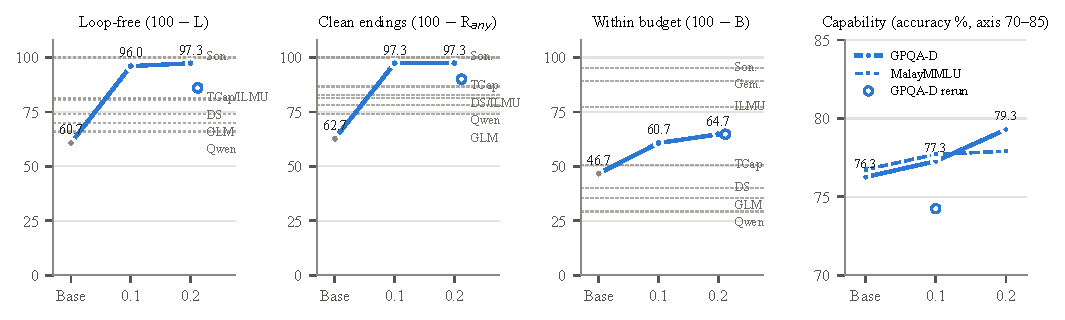
\includegraphics[width=\linewidth]{figures/trajectory.pdf}
  \caption{Base $\rightarrow$ Lamba 0.1 $\rightarrow$ Lamba 0.2 on g150 and on capability benchmarks; higher is better on every panel. Dashed lines are other models on the same test, for reference. The hollow marker in the first three panels is Lamba 0.2 at repetition penalty 1.0; in the last panel it is Lamba 0.1's second GPQA run. The capability panel uses a 70--85 axis.}
  \label{fig:traj}
\end{figure}

%=====================================================================
\section{Tool use and Lamba 0.2}
\label{sec:tools}
%=====================================================================

\subsection{Measuring redundant tool calls}

Every eval30 prompt asks the model to compute an exact value and then verify it, so the first verification call is required. Our first metric ignored that and reported that 37.5\% of runs ``ruminated''; it also counted crashed checks, legitimate repairs and follow-ups after a mismatch. The frozen metric (v2.2) defines a \emph{done point}: the exact value has appeared in a tool output and a successful call using the task family's independent verification method has completed. Calls after the done point are redundant. The metric was checked by hand on 13 labelled transcripts (all 5 flagged cases were correct; 2 known cases were missed) and parses fractions, LaTeX and Unicode minus signs. With it, redundant calls after verification are rare for most models (3--10\%).

\subsection{The sandbox was the main cause of tool failures}

In our original sandbox \verb|__import__| was blocked, and Lamba 0.1 never reached the correct answer in 37.5\% of runs on the 12 integral tasks. Every one of those runs involved import errors: the model expects \texttt{import} to work and spent its tool budget rediscovering that it does not. A sandbox that allows a whitelist of maths libraries (sandbox-B) rescued 29 of 36 such runs (80.6\%) within the original 8-round budget, with a median of 3 rounds. Stock Qwen3.8-27B failed at a similar rate (30.2\%) in the original sandbox, which points to the harness rather than the model. All eval30 numbers in this report use sandbox-B.

While building it we found that \texttt{sympify()} could execute arbitrary Python in both sandboxes. Tool code now runs inside a bubblewrap jail \citep{bwrap} with no network, a private filesystem and an empty environment, with the Python-level restrictions kept as a second layer.

\subsection{DPO stage}

Lamba 0.2 is a DPO \citep{rafailov2023dpo} stage on 406 preference pairs built from tool transcripts in which a runtime intervention had led the model to a correct answer. It is initialised from, and uses as its DPO reference, an earlier tool-use adapter trained on top of Lamba 0.1 (seed 1337, \S\ref{sec:pcr}). The loss is the DPO loss ($\beta=0.1$) plus an SFT term on chosen responses (weight 0.05), a KL term to a frozen copy of Lamba 0.1 on replay data (weight 0.10), a smaller KL term to Lamba 0.1 on the SFT rows (0.01), and a logit-matching regulariser (0.1). Training ran for 4 epochs (148 steps) at learning rate $5\times10^{-6}$. The pairs had a formatting error: the chosen side was only the final answer, without the reasoning block or end token, and the rejected side was flattened prose.

At repetition penalty 1.1 we found no significant difference between Lamba 0.2 and Lamba 0.1 on any eval30 metric, on g150, on GPQA-D (157 vs 153 and 147 correct; paired $p=0.54$ and $0.08$) or on MalayMMLU (77.91\% vs 77.71\%; $p=0.07$); see Tables~\ref{tab:versions} and \ref{tab:cross}. We did not pre-specify non-inferiority margins, so we describe this as ``no significant difference on the metrics tested''. On the integral-reconciliation family described next, where its initialisation adapter performed poorly in the original sandbox, Lamba 0.2 and Lamba 0.1 are both near zero in sandbox-B (Table~\ref{tab:pcrb}). At repetition penalty 1.0, Lamba 0.2 loops more ($\Rany$ 10.0\% vs 2.7\% at 1.1, paired $p=0.007$), so it is served at 1.1.

\subsection{An unshipped track: post-correct rumination}
\label{sec:pcr}

Two further adapters (seeds 1337 and 42) were trained to reduce tool-call rumination. Both passed our loop, capability and letter checks, but on a family of seven integral-reconciliation tasks, evaluated in the original sandbox that blocked imports, they more often reached the correct value and then kept calling tools until the budget ran out without answering (Figure~\ref{fig:pcr}). In that sandbox Lamba 0.1 did so in 16\% of runs and stock Qwen3.8-27B, a related untrained model, in 32.9\%. On eight non-integral tasks with the same structure (ODEs, series, linear systems and limits, 80 runs per adapter, same sandbox), Lamba 0.1 and both seeds were between 2.5\% and 6.2\% with no significant differences. Neither adapter shipped. A runtime guard that asks the model to stop and answer after a verified value is followed by calls that add no new information rescued 32 of 32 affected runs for seed 1337 and 14 of 14 on 12 held-out integrals, also in the original sandbox; it is not deployed.

\paragraph{The same family in sandbox-B.} We re-ran the integral family for the two shipped versions in sandbox-B, 70 runs each (7 tasks $\times$ 10). Post-correct rumination is essentially absent for both (Table~\ref{tab:pcrb}): 0 of 70 for Lamba 0.1 and 1 of 70 for Lamba 0.2 (Fisher exact $p=1.0$). The earlier 16\% for Lamba 0.1 was therefore a product of the restrictive sandbox, like the tool failures in \S\ref{sec:tools}. Lamba 0.2 does not improve on Lamba 0.1 here, and we do not claim that it does. The seed adapters were not re-run in sandbox-B, so their regression is established only in the original sandbox.

\begin{table}[t]
\centering
\small
\caption{Integral-reconciliation family in sandbox-B (70 runs per model). ``Overran then answered'': kept calling tools after reaching the value but still gave a final answer.}
\label{tab:pcrb}
\begin{tabular}{lccccc}
\toprule
Model & Post-correct rumination & Collapsed & Correct and stopped & Overran then answered & Budget hit \\
\midrule
Lamba 0.1 & 0/70 (0\%) & 0 & 39 & 31 & 2 \\
Lamba 0.2 & 1/70 (1.4\%) & 1 & 38$^\dagger$ & 28 & 1 \\
\bottomrule
\end{tabular}

\smallskip
\footnotesize $^\dagger$ Plus 3 runs correct only in the final answer.
\end{table}

\begin{figure}[t]
  \centering
  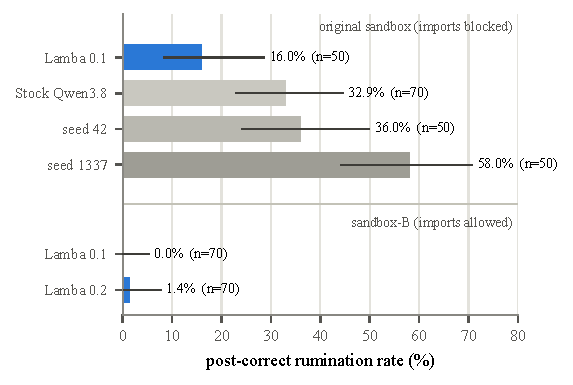
\includegraphics[width=0.5\linewidth]{figures/pcr_integral.pdf}
  \caption{Share of runs on integral-reconciliation tasks that reach the correct value and then exhaust the tool budget without answering, in the original sandbox that blocked imports. In sandbox-B the rate is 0\% for Lamba 0.1 and 1.4\% for Lamba 0.2 (Table~\ref{tab:pcrb}).}
  \label{fig:pcr}
\end{figure}

%=====================================================================
\section{Comparison with other models}
\label{sec:compare}
%=====================================================================

We ran eight other models on the same g150 and eval30 sets (Table~\ref{tab:cross}, Figure~\ref{fig:cross}). External models were called through their providers' APIs with temperature 0 on g150 where the provider accepts it. Our runner sets no reasoning-effort or thinking parameter for them, so each ran at its provider's default reasoning setting, and at provider-default repetition settings. Lamba, by contrast, runs at reasoning effort ``medium''. Claude models were run through Claude Code in headless mode with the same sandbox exposed as a tool server and extended thinking turned off; part of the Sonnet runs and its g150 run used the API directly, with the provider's default sampling and no thinking. For models that return reasoning in a separate field, we concatenated it with the answer before scoring. Lamba ran at repetition penalty 1.1, which the other models did not use, so the g150 comparison reflects each model as served rather than a matched decoding setup.

\begin{table}[t]
\centering
\small
\caption{g150 loop rates (\%, lower is better) and eval30 tool results: correct \%, redundant calls after verification (\% of runs reaching a verified answer, with that count $n_{\text{done}}$), assistant characters and tool calls per task.}
\label{tab:cross}
\setlength{\tabcolsep}{4.5pt}
\begin{tabular}{lcccc|ccccc}
\toprule
 & \multicolumn{4}{c|}{g150} & \multicolumn{5}{c}{eval30 (240 runs each)} \\
Model & $L$ & $\Rany$ & $\Rheavy$ & $B$ & Correct & Redund. & $n_{\text{done}}$ & Chars & Calls \\
\midrule
Lamba 0.2 & 2.7 & 2.7 & 0.0 & 35.3 & 98.8 & 8.8 & 160 & 1803 & 2.00 \\
Lamba 0.1 & 4.0 & 2.7 & 0.0 & 39.3 & 98.8 & 5.5 & 183 & 1793 & 1.92 \\
\midrule
Qwen3.8-27B (stock)$^a$ & 34.0 & 22.0 & 1.3 & 70.7 & 96.2 & 3.9 & 203 & 3084 & 1.34 \\
ThinkingCap-Qwen3.8-27B & 18.7 & 13.3 & 2.0 & 49.3 & 100 & 5.9 & 205 & 1171 & 1.43 \\
DeepSeek v4.1 Flash & 26.0 & 17.3 & 0.0 & 60.0 & 100 & 10.1 & 208 & 2023 & 1.78 \\
GLM-5.3 Flash & 30.0 & 26.0 & 8.0 & 64.7 & 91.2 & 3.2 & 188 & 5032 & 1.35 \\
ILMU v3.1 & 19.3 & 18.7 & 15.3 & 22.7 & 75.0 & 30.4 & 92 & 526 & 4.78 \\
Gemini 3.8 Flash$^b$ & -- & -- & -- & 10.7 & 100 & 4.1 & 197 & 885 & 1.18 \\
Claude Sonnet 5.5$^c$ & 0.0 & 0.0 & 0.0 & 4.7 & 100 & 0.0 & 57 & 540 & 1.16 \\
Claude Opus 5.5$^c$ & -- & -- & -- & -- & 100 & 1.7 & 59 & 722 & 1.04 \\
\midrule
\multicolumn{10}{l}{\emph{Matched decoding: repetition penalty 1.1 for all}} \\
Base model (no adapter) & 8.7 & 4.7 & 0.0 & 36.0 & & & & & \\
Qwen3.8-27B (stock) & 22.0 & 10.0 & 0.0 & 66.0 & & & & & \\
ThinkingCap-Qwen3.8-27B & 11.3 & 7.3 & 0.7 & 38.0 & & & & & \\
\bottomrule
\end{tabular}

\smallskip
\footnotesize $^a$ A second run of stock Qwen through a different provider gave $L$ 36.0, $\Rany$ 20.7, $\Rheavy$ 0.0, $B$ 74.0. $^b$ Reasoning is not returned, so repetition cannot be scored. $^c$ Without extended thinking; Opus was not run on g150. GLM, DeepSeek and Gemini are their providers' fast-tier models. Redundancy rates rest on very different $n_{\text{done}}$ and are not directly comparable across models.
\end{table}

\begin{figure}[t]
  \centering
  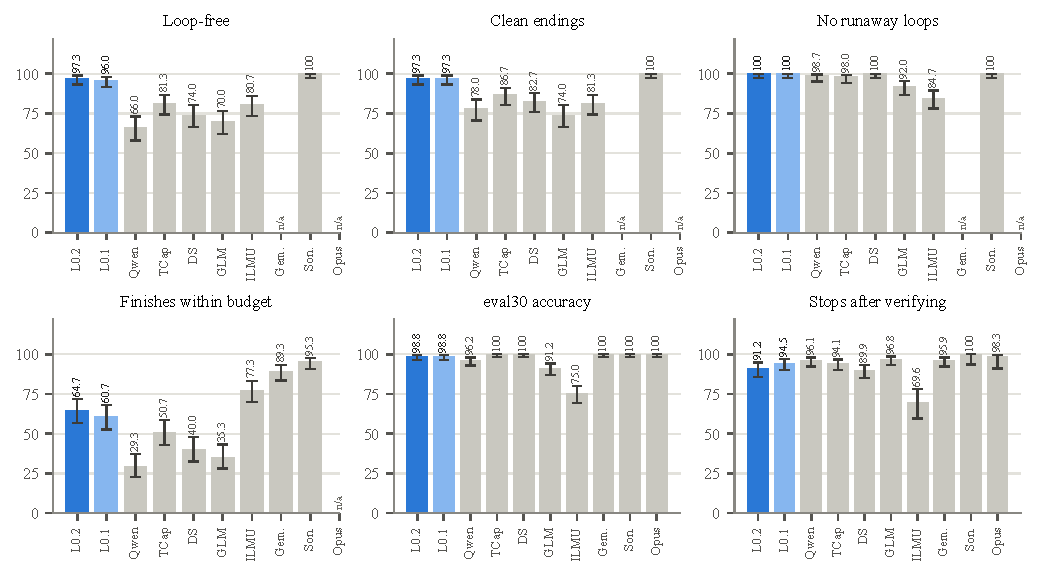
\includegraphics[width=\linewidth]{figures/crossmodel.pdf}
  \caption{Table~\ref{tab:cross} as ``higher is better'' scores (100 minus each rate), with 95\% Wilson intervals (150 prompts for g150, 240 runs for eval30 accuracy, $n_{\text{done}}$ runs for redundancy; eval30 intervals ignore clustering by task and are therefore too narrow). Lamba 0.2 and 0.1 in blue.}
  \label{fig:cross}
\end{figure}

On g150, Lamba as served has lower loop rates than the other open-weight models in the table; Claude Sonnet 5.5 has the lowest. On $\Rheavy$, the strictest metric, Lamba 0.1 is level with DeepSeek and stock Qwen and lower than GLM ($p=0.0005$). Because the penalty alone does much of the work (\S\ref{sec:decoding}), we also ran the two same-architecture models at penalty 1.1 (bottom of Table~\ref{tab:cross}). The penalty helps them too, but at matched decoding Lamba 0.2 still has fewer Liquid-style loops than stock Qwen (4 vs 33 of 150, $p=10^{-6}$) and ThinkingCap (4 vs 17, $p=0.004$) and fewer budget hits than stock Qwen (53 vs 99, $p=3\times10^{-10}$). Against ThinkingCap at 1.1, the differences in tail repetition (4 vs 11, $p=0.09$) and budget hits (53 vs 57) are not significant. On eval30, accuracy is near the ceiling for most models, and Lamba writes 1.5 to 3.3 times more text per task than Claude, Gemini and ThinkingCap and makes more tool calls. ThinkingCap \citep{thinkingcap} hits the 4,000-token cap more often than Lamba 0.2 (49\% vs 35\%), but on prompts both finish its median length is about 740 tokens against 1,661 for Lamba 0.2. Closing this gap likely needs training with a correctness reward and a length cost.

%=====================================================================
\section{Analysis: what the training changes}
\label{sec:analysis}
%=====================================================================

\paragraph{Training and the penalty overlap, and stack.} Table~\ref{tab:decoding} shows the two levers reach similar end points by different routes. The penalty acts on every token at every step, with no change to the model; training changes the model's preferences at loop onsets and leaves decoding untouched. On their own each removes nearly all runaway loops, and their effects add up on the shorter repeats that remain: training on top of the penalty removes about 60\% of what the penalty alone leaves. A plausible reading is that the penalty makes repetition expensive everywhere while FTPO makes the model less inclined to start a repeat in the first place; we have not tested this mechanism directly. The practical difference is robustness: a trained model does not depend on users applying the right decoding setting, while the penalty has a narrow useful window (Figure~\ref{fig:rp}: 1.15 already helps less than no penalty, and 1.2 is worse than the base model).

\paragraph{The training data are mostly re-quoting loops, and the effect transfers.} Of the 1,298 first-round pairs, 1,038 (80\%) come from loops whose repeated window also appears in the prompt: the model restating the question or an option over and over. Our evaluation discards windows that occur in the prompt, so every reduction we report is in text the model wrote itself. The reduction also holds on science and Malay prompts, which share little wording with training prompts: Liquid-style loops fall from 43 to 5 of 85 (Table~\ref{tab:domain}).

\paragraph{The training position decides the outcome.} The first pipeline cut the context one occurrence too early, at the start of the first occurrence. The rejected tokens were then ordinary text (15\% were \verb|\n\n|), and training cut the newline rate from 7.11 to 0.03 per 1,000 characters and increased looping. Moving the position to the second occurrence, as Algorithm~\ref{alg:mining} does, is the difference between the failed and the working adapters.

\paragraph{Loops depend on the whole trajectory.} We took looping outputs from one of the adapters of our KL-tie experiments (\S\ref{sec:negative}). At the onset of a loop, that adapter and Lamba 0.1 disagree \emph{less} than elsewhere in the same output (7 of 8 cases), and Lamba 0.1 itself loops in 67\% of cases when continued from the same prefix, whether it takes over at the onset or up to 100 tokens earlier. A loop is therefore not a single bad token that a local fix can repair: by the time it starts, the context already pulls strongly towards it, consistent with the self-reinforcement described by \citet{xu2022ditto}. Training works by making the model less likely to enter such states, not by correcting them at one point.

\paragraph{Why stronger penalties fail.} The penalty lowers the logit of every token already used, which includes the words and symbols a long answer needs. On malay-final, budget hits are 41.3\% at penalty 1.0, 36.7\% at 1.1, 50.7\% at 1.15 and 86.7\% at 1.2, and mean output length at 1.2 is more than twice that at 1.0 (17,723 vs 7,879 characters). Beyond 1.1 the model cannot finish; the primary endpoint at 1.2 is worse than the base model's (Figure~\ref{fig:rp}).

\paragraph{Seed robustness.} We retrained the last loop stage (v9c) with a different seed, keeping its initialisation and data. Table~\ref{tab:seed} shows no significant difference on any loop or capability metric. Earlier stages were trained once, so this measures the variance of the final stage only. The two tool-rumination seeds in \S\ref{sec:pcr} are a reminder that seed variance can matter: they behaved very differently on the integral family in the original sandbox.

\begin{table}[t]
\centering
\small
\caption{Seed replication of the v9c stage (repetition penalty 1.0, g150). Paired exact McNemar $p$ for loop metrics.}
\label{tab:seed}
\begin{tabular}{lccccccc}
\toprule
 & $L$ & $\Rany$ & $\Rheavy$ & $B$ & MalayMMLU & A--B gap & GPQA-D \\
\midrule
v9c (seed 3407) & 22.7 & 16.7 & 2.7 & 41.3 & 76.50 & $-12.6$ & 154/198 \\
v9c (seed 2) & 18.0 & 15.3 & 2.7 & 42.0 & 76.51 & $-13.0$ & 157/198 \\
$p$ & 0.23 & 0.83 & 1.0 & 1.0 & -- & -- & -- \\
\bottomrule
\end{tabular}
\end{table}

%=====================================================================
\section{Negative results}
\label{sec:negative}
%=====================================================================

\begin{itemize}
  \item \textbf{Tying a shortening run to Lamba 0.1.} SFT on naturally concise correct outputs gave the best capability numbers of any adapter (GPQA-D 162/198) but increased loops. A KL tie to Lamba 0.1 kept the length reduction and lowered the loop cost, but across three seeds the excess loop rate did not reliably stay under the 2-point cap; the effect of the tie strength was smaller than seed-to-seed variation.
  \item \textbf{Length-conditioned repetition penalty.} A decode-time penalty that activates once the output is long and a repeated n-gram is detected was harmful as a replacement for the fixed penalty ($\Rany$ +29.7 points on science) and neutral to harmful as an addition.
  \item \textbf{Local repair of loops.} Training on Lamba 0.1's continuation at the onset of another adapter's loops was not viable: those continuations also loop in 67\% of cases, and starting up to 100 tokens earlier did not help (\S\ref{sec:analysis}).
  \item \textbf{Structural loops.} Prompts designed to elicit enumeration or rumination loops yielded 2 genuine cases in 486 (0.4\%); we stopped.
  \item \textbf{Efficient reasoning.} A 378-pair Malay pilot reduced budget hits by 8 points ($p=0.023$) without loop regression. Two cross-domain expansions, which chose the stopping point by probing for a correct forced answer, increased $\Rany$ to 17.3\% and 26.0\%: on multiple-choice data, forced early answers are often right by chance, so the method taught the model to stop too early. The pilot used outputs from other models as reference lengths and was not shipped.
  \item \textbf{Seed adapters for tool rumination} (\S\ref{sec:pcr}). Not shipped.
\end{itemize}

%=====================================================================
\section{Findings from live use}
%=====================================================================

\paragraph{The original incident.} The prompt that started the investigation was a short question about a Latin phrase. Lamba 0.1 reasoned at length, described itself with a persona and instructions it had not been given, and ended without an answer. Lamba 0.2 answered the same prompt in a few lines. On 60 prompts of the same kind, blind-labelled and then hand-audited, invented identity or instructions appeared in 6 of 60 Lamba 0.1 answers and 3 of 60 Lamba 0.2 answers (Fisher $p=0.49$). The raw labeller counts were 11 and 3 ($p=0.043$) before an audit that was designed after seeing them.

\paragraph{Identity.} Without a system prompt, Lamba 0.2 does not identify itself as Lamba and in 96\% of cases names another model, most often Qwen. With our system prompt it says Lamba 88\% of the time. When a client supplies its own system prompt, our server now presents it as application instructions, which helped in a small test (3/4 to 4/4).

\paragraph{Tool follow-through.} On 248 held-out prompts at temperature 1.0, Lamba 0.2 calls a tool in 71.8\% of cases where one is warranted. It announces a search and then ends its turn without calling the tool in 2.4\% of cases, and answers questions about obscure entities without searching in 25.8\%.

%=====================================================================
\section{Lessons for practitioners}
%=====================================================================

\begin{enumerate}
  \item \textbf{Get the training position exactly right.} AntiDoom only worked once pairs were taken at the start of the \emph{second} occurrence. One position earlier, the same pipeline taught the model to stop writing newlines.
  \item \textbf{Mine from the model's own outputs, per domain.} Each round on the adapter's own loops removed loops the previous round left behind, and Malay needed its own round. Where natural loops are rare, model-written prompts with real rollouts supply enough examples.
  \item \textbf{Run the decoding-only baseline first.} A repetition penalty on the untouched base model turned out to do about as much as our training. Running that baseline at the start, and the full $2\times2$ of model and decoding, is what tells you what training is actually for.
  \item \textbf{Select bias checkpoints on large held-out data.} A 664-question validation set showed a stable 2--6 point gap while the full benchmark swung by 25 points across the same checkpoints.
  \item \textbf{Check the harness before blaming the model.} Most of Lamba 0.1's tool failures, and stock Qwen's, came from a sandbox that blocked imports; so did its 16\% rate of post-correct rumination on integrals, which falls to 0\% in a working sandbox.
  \item \textbf{Hand-check and freeze every metric.} Four rounds of real bugs were found by reading fresh outputs, including the detector substitution reported in Table~\ref{tab:primary}.
\end{enumerate}

%=====================================================================
\section{Limitations}
\label{sec:limits}
%=====================================================================

\begin{itemize}
  \item \textbf{The penalty does much of the work.} A repetition penalty alone gives a loop reduction comparable to our training (Table~\ref{tab:decoding}); the adapters' added value at the serving setting is a further reduction of the remaining short repeats, not of budget hits or the primary endpoint. We did not measure the capability cost of the penalty on the base model.
  \item \textbf{Detector choice.} The pre-registered endpoint misses its relative target on the best-powered test. Our loop detectors are our own, and the Liquid-style detector belongs to the same family as the one used to mine training pairs. The independent checks ran on earlier adapters, and the blind adjudication used a single model as annotator.
  \item \textbf{Selection on test sets.} The repetition penalty was chosen on g150, and the letter-bias checkpoint on the full MalayMMLU.
  \item \textbf{Scale.} One base model, one GPU, 150 to 700 prompts per loop comparison, mostly greedy decoding; one sampled check on 100 prompts agrees.
  \item \textbf{Capability checks.} GPQA-D was run from an ungated mirror with a 4,000-token budget, so 51--59\% of answers are cut off. There is no code-domain evaluation, and the tool evaluation is maths only.
  \item \textbf{Lamba 0.2.} No pre-specified non-inferiority margins. The seed adapters' integral regression was measured only in the original sandbox and was not re-run in sandbox-B.
  \item \textbf{Generality.} All results are on one base model that we continued training ourselves; we have not shown the recipe transfers to other bases. Lamba 0.4 uses a different base and a different training pipeline, so it is not a clean test of transfer, and comparisons between the two reports mix changes in base and in training.
\end{itemize}

%=====================================================================
\section{How this work was done}
%=====================================================================

Most of the engineering, data generation and labelling was done with two AI systems, while we set the goals and made every ship decision. DeepSeek v4.1 Flash wrote prompt sets, labelled transcripts blind and drafted code. Claude (Opus and Sonnet) planned experiments, checked designs and results, and ran the machine. Errors in proposals from both were caught and corrected along the way; the ones that affected reported numbers are listed in Appendix~\ref{app:retractions}.

%=====================================================================
\section{Conclusion}
%=====================================================================

With one GPU and two weeks, a port of AntiDoom mined on the adapter's own outputs and separately per language removed nearly all runaway loops from a 28.8B hybrid Gated DeltaNet model without any change to decoding. A repetition penalty of 1.1 achieves a similar reduction on the untouched base model, and the two together leave the fewest loops of any configuration we tested, fewer than same-architecture models at the same penalty. The pre-registered loop endpoint improved significantly under every configuration, though not by the 30\% we targeted. A group-level permutation objective reduced the answer-letter gap substantially, with the caveat that the checkpoint was chosen on the benchmark used to report it. Capability was unchanged within noise. The main open questions are whether the letter result holds on held-out data and how to reduce verbosity, which we expect to need reinforcement learning with a length cost. The identity and tool-use weaknesses found in live use are addressed in Lamba 0.3 and 0.4, which continue this work and are described in a separate report.

\paragraph{Release.} Lamba 0.1 and 0.2 are internal research versions and their weights are not released. Lamba 0.4, the version we do release as open weights, is described together with Lamba 0.3 in a separate report, which continues the line of work set out here. What accompanies this report is code: the trainer and its configurations, the mining scripts, the loop and tool evaluation harnesses, and the scoring scripts named in the Reproduction section. We do not release raw model outputs, training data or our internal working notes. The code is at \url{https://github.com/Vix0007/lamba}, and the Lamba 0.4 weights and model card are at \url{https://huggingface.co/VixeroAI/Lamba-0.4}.

\paragraph{Author contributions.} One researcher at Vixero Labs set the goals, designed and ran all experiments, wrote the evaluation protocols and made every ship decision. AI systems assisted with engineering, data generation, labelling and drafting, as described in the section ``How this work was done''; they are not authors.

\paragraph{Broader impact.} Fewer runaway loops mean fewer wasted tokens and fewer answers that never arrive, and the Malay work improves a lower-resource language. Lamba still answers questions about obscure entities without checking in about a quarter of cases and does not reliably know its own identity without a system prompt; the model card states both. We do not release benchmark items: GPQA question text is withheld. Lamba is built on a Qwen-family base, as its model card states.

\bibliographystyle{plainnat}
\bibliography{refs}

\appendix

%=====================================================================
\section{Corrections}
\label{app:retractions}
%=====================================================================

The following numbers appeared in internal notes and were corrected.

\begin{itemize}
  \item \textbf{Primary endpoint detector.} Internal summaries reported the primary endpoint computed with the Liquid-style detector (e.g.\ 31.2\% on 700 prompts) as the pre-registered result. With the pre-registered detector the figure is 22.8\% (Table~\ref{tab:primary}).
  \item \textbf{Loop reduction attributed to training.} Earlier drafts credited the full reduction from the base model to the adapter at penalty 1.1. A penalty-only baseline shows the penalty alone achieves a comparable reduction; the adapter's further contribution at the serving setting is limited to the remaining short repeats (\S\ref{sec:decoding}).
  \item \textbf{Integral-family rumination.} The 16\% rate for Lamba 0.1 came from a sandbox that blocked imports; in sandbox-B it is 0 of 70 (Table~\ref{tab:pcrb}).
  \item \textbf{``Lamba 0.2 is 30\% less verbose than 0.1.''} The 0.2 model folder linked to the base model's generation settings, which lack the repetition penalty, so it was evaluated at 1.0 while 0.1 ran at 1.1. At matched settings they do not differ significantly.
  \item \textbf{``Tool rumination 37.5\%.''} A metric artifact; see \S\ref{sec:tools}. (Unrelated to the 37.5\% of runs that never reached the answer in the original sandbox.)
  \item \textbf{Sandbox rescue rate 82.1\%.} A number-matching bug omitted one-decimal answers on five tasks. The corrected rate, for a predecessor adapter combined with sandbox-B, is 94.6\%.
  \item \textbf{``Stock Qwen shows 0\% repetition.''} Its reasoning was stored in a separate field the scorer did not read.
  \item \textbf{``0.2's predecessor halves rumination versus 0.1.''} True only in the original sandbox.
  \item \textbf{Latin-incident counts.} An early labelling prompt wrongly stated that the system prompt contained nothing about identity. Counts were redone with a corrected rubric.
  \item \textbf{A third guard failure mode.} Empty answers in a synthetic stress test came from artificial tool-call identifiers in the test itself; with real identifiers the failure did not occur.
  \item \textbf{Sonnet 5.5 eval30.} An early partial run (0 of 35 redundant, 501 characters, 1.19 calls) was superseded by the full 240 runs in Table~\ref{tab:cross}.
  \item \textbf{Mean length under a hard cap.} Truncated outputs pull the mean down; length comparisons use paired medians on prompts both models finish.
\end{itemize}

%=====================================================================
\section{Training details}
\label{app:hparams}
%=====================================================================

All stages use NF4 QLoRA with the adapter layout of \S3, batch size 1 with gradient accumulation, AdamW and a learning-rate warmup over 5--10\% of steps. Loop and letter stages use a maximum sequence length of 6,000 tokens; the tool stages use 8,000 and 20,000.

\begin{table}[h]
\centering
\small
\setlength{\tabcolsep}{4pt}
\begin{tabular}{>{\raggedright\arraybackslash}p{2.0cm}>{\raggedright\arraybackslash}p{2.6cm}>{\raggedright\arraybackslash}p{5.2cm}ccc}
\toprule
Stage & Initialised from & Training data & Epochs & LR & Eff.\ batch \\
\midrule
v8 & base & 1,298 FTPO pairs (filtered AntiDoom events) & 2 & $1.5\times10^{-5}$ & 16 \\
v9b & v8 (via an intermediate run) & 909 own-output rows (hard + soft) + 120 base-tie rows & 2 & $2\times10^{-5}$ & 16 \\
v9c & as v9b & v9b data + 1,080 letter-tie rows & 2 & $2\times10^{-5}$ & 16 \\
malay-final & v9c & 273 Malay rows (weight 0.25) + 600 replay + 200 letter-tie & 1 & $1\times10^{-5}$ & 16 \\
Lamba 0.1 & malay-final & 1,080 rotation groups; step 10 kept & 2 & $1\times10^{-5}$ & 16 \\
Seed 1337 & Lamba 0.1 & about 190 rows: 29 targeted rows (tool rumination, confabulation) + replay ties & 2 & $2\times10^{-5}$ & 16 \\
Lamba 0.2 & seed 1337 & 406 DPO pairs + 800 replay rows & 4 & $5\times10^{-6}$ & 32 \\
\bottomrule
\end{tabular}
\end{table}

Loss settings: FTPO stages use a logit-clip margin of 1.5 and a logit-matching tether to the base model (weight 2.0 for v8, 0.1 afterwards) with gradient clipping at 5. The letter stage uses hinge 0.4, permutation variance 0.2 and entropy 0.05. Lamba 0.2's loss is given in \S\ref{sec:tools}.

%=====================================================================
\section{Compute}
\label{app:compute}
%=====================================================================

Everything ran on one NVIDIA L40S (48\,GB) with 30\,GB of host RAM, with a second L40S for evaluation on a few days. Training stages took between about 15 minutes and a few hours, except the DPO stage of Lamba 0.2, which took 10.5 hours. One g150 evaluation of an adapter takes about an hour, the full MalayMMLU about 20 minutes and GPQA-D about 75 minutes. The work from the first training run to Lamba 0.2, including all failed attempts, took two weeks of wall-clock time on this hardware.

%=====================================================================
\section{Reproducibility checklist}
%=====================================================================

\begin{itemize}
  \item \textbf{Do the claims match the results?} Yes. The headline loop claims are stated per metric, and the pre-registered endpoint is reported under the planned and the substituted detector (Table~\ref{tab:primary}).
  \item \textbf{Are limitations discussed?} Yes, in \S\ref{sec:limits}, including selection on test sets.
  \item \textbf{Statistical significance.} Paired comparisons use exact McNemar tests; relative reductions carry 95\% bootstrap intervals (2,000 resamples over prompts); Figures~\ref{fig:lineage} and \ref{fig:cross} show 95\% Wilson intervals. With 150 prompts, a rate near 20\% has an interval of roughly $\pm$6 points.
  \item \textbf{Seeds.} The final loop stage was replicated with a second seed (Table~\ref{tab:seed}); other stages were trained once.
  \item \textbf{Pre-registration.} The loop endpoint was fixed before training; one amendment was made before any adapter data were seen, and one detector substitution was made later and is disclosed.
  \item \textbf{Code, data and outputs.} We release the trainer, configurations, mining scripts, evaluation harnesses and scoring scripts. We do not release raw model outputs, training data, or the weights of Lamba 0.1 and 0.2, so the numbers in this report can be re-derived by running the released harness on a model, not recomputed from our outputs. GPQA question text is withheld.
  \item \textbf{Compute.} Appendix~\ref{app:compute}.
\end{itemize}

%=====================================================================
\section{Prompts and harness}
\label{app:prompts}
%=====================================================================

\paragraph{g150 loop test.} Each prompt is sent as a single user message with no system prompt, through the model's chat template, greedy, with a 4,000-token cap. Prompts are released in \texttt{antidoom\_data/}\allowbreak\texttt{loop\_testset150.jsonl}.

\paragraph{eval30 tool test.} Every model, including the external ones, receives the same system prompt (Lamba's serving prompt: an identity line, the current date and the Lamba constitution) and the same two tools, so the harness is identical across models. The tool used in every task is:

\begin{quote}\small\ttfamily\raggedright
python\_eval: Execute Python code in a sandbox with sympy pre-imported (all its names available directly, e.g. symbols, Matrix, simplify, expand, solve, nsimplify). Use this for any exact symbolic math, arithmetic, or verification -- never do hand algebra you can instead compute exactly. No filesystem, network, or OS access; 15s CPU/wall-clock limit, 1GB memory limit. Use print() for output.
\end{quote}

A web-search tool is also offered but is not needed for any task. Two example task prompts:

\begin{quote}\small
\emph{Integral:} ``Using python\_eval with SymPy, compute the definite integral of 1/(x\^{}2+4) from x=0 to x=2, then verify by numerically integrating the same function over the same bounds (e.g.\ via a fine Riemann sum or sympy's numerical integration) and confirming the two match.''

\emph{ODE:} ``Using python\_eval with SymPy, solve the ODE y'' + y = 0 with y(0)=0, y'(0)=1 exactly and report y(1). Then verify by numerically integrating the ODE (e.g.\ a hand-written RK4 loop or scipy solve\_ivp) from 0 to 1. Report the final value of y(1).''
\end{quote}

Runs use temperature 0.8, top-$p$ 0.95 and seed equal to the repetition index, with at most 8 tool rounds followed by one forced answer turn without tools. The Claude Code harness runs at most 9 turns and has no forced answer turn; this never came into play.

\paragraph{GPQA-Diamond.} The system message reads: ``Reasoning effort is set to xhigh. Please think carefully through the task, validate key assumptions, consider plausible alternatives, and prioritize correctness, consistency, and clarity in the final answer.'' The user message contains the question and lettered options. At the 4,000-token budget the reasoning is cut and the model is asked for its answer. Question text is not reproduced here.

\paragraph{MalayMMLU.} Each item uses the benchmark's prompt (the question and its lettered options, one per line) followed by ``Answer:''; the prediction is the option letter with the highest log-probability as the next token.

%=====================================================================
\section{Reproduction}
%=====================================================================

\begin{itemize}[before=\raggedright]
  \item Loop test: \texttt{antidoom\_data/loop\_test\_g.py}; loop metrics with \texttt{tail\_stats\_cmp.py}, which refuses to compare files generated at different repetition penalties; the pre-registered endpoint with \texttt{loop\_compare\_v2.py}.
  \item Tool test: \texttt{gen\_sandboxb\_eval.py} for local models, \texttt{gen\_ilmu.py} for API models, \texttt{gen\_claude\_sub.py} for Claude Code; scoring with \texttt{rumination\_metric\_v2\_2\_FROZEN.py}.
  \item Training configurations: \texttt{antidoom\_src/configs/}; Lamba 0.2 uses \texttt{lamba\_ruminconfab\_dpo\_v2.yaml}.
  \item Figures in this report: \texttt{report/make\_figures.py}.
\end{itemize}

\end{document}
